\documentclass[compress]{beamer}

\usepackage[nofonts]{ctex}
\setCJKmainfont[ItalicFont={Kaiti SC}]{Kaiti SC}%
%\setCJKmainfont[ItalicFont={AR PL KaitiM GB}]{AR PL KaitiM GB}%
%\setCJKsansfont{WenQuanYi Zen Hei}% 文泉驿的黑体

\mode<beamer>
{
    \setbeamercovered{transparent}

    \useinnertheme{rounded}
    %\useoutertheme{miniframes}
    \useoutertheme{split}
    %\usecolortheme{orchid}
    %\usecolortheme{whale}
    %\usecolortheme{lily}
    \usecolortheme{rose}
    \usecolortheme{seahorse}

	\expandafter\def\expandafter\insertshorttitle\expandafter{%
	\insertshorttitle\hfill%
	\insertframenumber\,/\,\inserttotalframenumber}
}

\mode<handout>
{
	\usetheme{default}
	\usepackage{pgfpages}
	\pgfpagesuselayout{4 on 1}[a4paper,landscape,border shrink=5mm]
}


\usepackage{amsmath,latexsym,amssymb,amsfonts,amsbsy}
\usepackage{graphicx}
\usepackage{hyperref}
\usepackage{ulem}
\usepackage{fancyvrb}
\fvset{frame=single,numbers=left, tabsize=4,fontsize=\footnotesize}
\usepackage{tikz}
\usetikzlibrary{calc, arrows.meta, shapes, positioning, automata}

\newcommand{\romannumber}[1]{{\textrm{\uppercase\expandafter{\romannumeral
#1}}}}
\setbeamercolor{dblue}{fg=white,bg=blue!40!black} % for beamercolorbox
\newenvironment{pblock}{\begin{beamercolorbox}[rounded=true,
                              shadow=true]{dblue}}{\end{beamercolorbox}}


\graphicspath{{figure/}}

%%%%%%%%%%%%%%%%%%%%%%%%%%%%%%%%%%%%%%%%%%%%%%%%%%%%%%%%%%%%%%%%%
%    body                                                       %
%%%%%%%%%%%%%%%%%%%%%%%%%%%%%%%%%%%%%%%%%%%%%%%%%%%%%%%%%%%%%%%%%


\begin{document}

\AtBeginSection[]
{ 
    \begin{frame}<beamer> 
		\frametitle{内容提要} 
		\tableofcontents[currentsection,currentsubsection] 
	\end{frame} 
} 
					
\title{高级编程工具}

\author[\href{http://c.pku.edu.cn/}{http://c.pku.edu.cn/}]
{曹东刚\\\href{mailto:caodg@sei.pku.edu.cn}{caodg@sei.pku.edu.cn}}

\institute{Linux程序设计环境 \\
\href{http://c.pku.edu.cn/}{
http://c.pku.edu.cn/}}

\date{}

\titlegraphic{\includegraphics[height=0.17\textwidth]{Overlays/logo.pdf}}

\begin{frame}
	\titlepage
\end{frame}

\section{lex and yacc}

\begin{frame}
\frametitle{yacc}
\begin{itemize}
\item \alert{Yacc}: ``Yet Another Compiler Compiler''\\
是 Unix 系统中标准的生成语法分析程序的程序

    \begin{itemize}
    \item 基于 BNF 范式
    \item 生成 C 语言代码
    \item 生成的语法分析程序需要一个词法分析器 (lexical analyzer)
    \end{itemize}
\item 多种 \alert{Yacc} 工具, 如 GNU 的 \alert{bison}
\end{itemize}


\end{frame}

\begin{frame}
  \frametitle{lex}

\begin{itemize}
\item \alert{lex} 是Unix 系统中标准的生成词法分析器的程序
\item IEEE POSIX P1003.2 对 \alert{Lex} 和 \alert{Yacc} 进行了标准化
\item 多种 \alert{Lex} 工具, 如 GNU 的 \alert{flex}
\end{itemize}

\end{frame}

\begin{frame}
\frametitle{flex}

\begin{itemize}
  \item {flex} 基于\uline{有限状态识别机}生成词法分析器

  \item {flex} 输入文件通过若干\uline{规则}描述词法分析器
    \begin{itemize}
    \item 规则: 正则表达式和对应的C 代码
    \end{itemize}

\item {flex} 缺省生成一个名为 `lex.yy.c' 的C文件, 
  该文件的 `yylex()' 函数扫描输入文本

\item 编译该文件并和库 \alert{libfl.a/libl.a} 链接, 生成可执行文件

\item 该文件执行时, 对遇到的每一个规则, 执行对应的 C 代码
\end{itemize}

\end{frame}


\begin{frame}
\frametitle{Finite States Recognizers}

FSR是一种\uline{有限自动机}, 定义了若干接受状态(accepting states).
如果存在一条路径从初始状态到接受状态, 则称输入可接受.\\
例: 识别程序文本中的``go to'', ``goto''\\[2ex]

  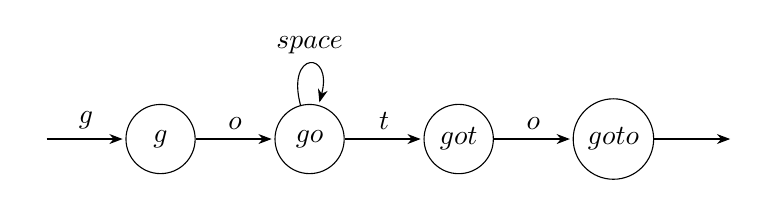
\begin{tikzpicture}[shorten >=1pt,>=Stealth, node distance=1cm,auto]
    \node (g0) {};
    \node[state,right = of g0] (g) {$g$};
    \node[state,right = of g] (go) {$go$};
    \node[state,right = of go] (got) {$got$};
    \node[state,right = of got] (goto) {$goto$};
    \node[right = of goto] (g1) {};

    \path[->] (g0)  edge    node        {$g$} (g)
              (g)   edge    node        {$o$} (go)
              (go)  edge    node        {$t$} (got)
                    edge [loop above] node {$space$} ()
              (got) edge    node        {$o$} (goto) 
              (goto)    edge    (g1);
  \end{tikzpicture}
\end{frame}

\begin{frame}
\frametitle{生成的词法分析程序工作过程 ---1 }
\begin{itemize}
\item 读取输入, 对输入字符串搜寻匹配的模式
    \begin{itemize}
    \item 若发现多个匹配模式, 则选择匹配最长字符串的那个
    \item 若模式匹配字符串长度相同, 则选择第一个模式
    \end{itemize}
\end{itemize}

\end{frame}


\begin{frame}
\frametitle{生成的词法分析程序工作过程 ---2 }
\begin{itemize}
\item 确定匹配模式后
    \begin{itemize}
    \item 全局字符串指针 ``yytext'' 指向匹配字符串, 全局变量 ``yyleng''定义了字符串长度
    \item 执行该模式的关联动作
    \end{itemize}
  \item 若没有发现匹配模式, 则执行缺省动作: \uline{将输入复制到输出}
\end{itemize}
\end{frame}

\begin{frame}[containsverbatim]
\frametitle{flex输入文件规格}

{flex}输入文件由3部分组成
\begin{itemize}
  \item 定义
  \item 规则
  \item 用户代码
\end{itemize}
每部分之间由\verb~ %% ~ 分隔


\end{frame}

\begin{frame}[containsverbatim]
\frametitle{flex输入文件模板}
\begin{Verbatim}[label=flex 模板]
%{
user-file-prologue
%}
definitions
%%
%{
user-yylex-prologue
%}
regular-expression-1 action-1
...
%%
user-epilogue
\end{Verbatim}
\end{frame}

\begin{frame}[containsverbatim]
\frametitle{flex输入文件例子}
\begin{Verbatim}[label=flex示例]
%{
int num_lines = 0, num_chars = 0;
%}
%%
\n      ++num_lines; ++num_chars;
.       ++num_chars;

%%
main()
{
    yylex();
    printf( "# of lines = %d, # of chars = %d\n",
            num_lines, num_chars );
}
\end{Verbatim}
\end{frame}

\begin{frame}[containsverbatim]
\frametitle{定义部分}

为了简化输入文件, 可以在定义部分声明若干名字定义, 以及若干开始条件.
名字定义的形式为\\
\verb~name definition~\\
其中 \\
name: \verb~[a-zA-Z_][a-zA-Z0-9_-]*~ \\
definition: 从name后第一个非空白字符开始至行尾\\
可通过\verb~{name}~引用definition. 例:\\
\begin{Verbatim}
DIGIT    [0-9]
ID       [a-z][a-z0-9]*
FLOAT    {DIGIT}+"."{DIGIT}*
\end{Verbatim}
\end{frame}

\begin{frame}[containsverbatim]
\frametitle{规则部分和用户代码部分}

\begin{itemize}
\item 规则部分定义了若干``模式--动作''对\\
\verb~pattern   action~\\
其中``pattern''前面不能有缩进, ``action''必须和``pattern''在同一行
\item 用户代码部分被复制到生成的文件 `lex.yy.c'中
  \begin{itemize}
	\item 在此部分可以定义调用词法分析器/被词法分析器调用的函数, 如``main''函数
	\item 如果没有用户代码, 在此部分连同前面的\verb~%%~无需声明
\end{itemize}
\end{itemize}
\end{frame}

\begin{frame}[containsverbatim]
  \frametitle{最简单的{flex}定义}

\verb~%%~

\end{frame}

\begin{frame}[containsverbatim]
\frametitle{prologue}

在定义部分和规则部分可以定义序言(prologue)\\
prologue: 缩进文本或`\verb~%{~'与 `\verb~}%~'之间的文本 \\
`\verb~%{~'与 `\verb~}%~'不能缩进

\begin{itemize}
  \item 定义部分的序言常用于声明\uline{全局变量}, 规则动作要用到的
    \uline{头文件}等\\
定义部分的序言被{flex}复制到生成的文件`lex.yy.c'中
\item 规则部分的序言在规则部分开始声明\\
  规则部分的序言定义词法分析器用到的\uline{局部变量}, 词法分析器的
  \uline{初始化动作}等
\end{itemize}

\end{frame}

\begin{frame}[containsverbatim]
\frametitle{规则}
规则部分使用扩展的正则表达式\\[1ex]
{\footnotesize
\begin{tabular}{|l|p{8cm}|}\hline
\verb~x~ & 匹配字符`x' \\ \hline
\verb~.~ & 匹配除换行外的任意单个字符 \\ \hline
\verb~[xyz]~ & 匹配方括号中的任意字符 \\ \hline
\verb~[abj-oZ]~ & 匹配字符`a', `b', 从`j'到`o'的字符, 或`Z' \\ \hline
\verb~[^A-Z]~ & 不匹配从`A'到`Z'的字符 \\ \hline
\verb~[^A-Z\n]~ & 不匹配从`A'到`Z'的字符以及换行符 \\ \hline\hline
\verb~{name}~ & 引用定义部分定义的模式 \\ \hline
\verb~r*~ & r是正则表达式, 匹配r任意多次 \\ \hline
\verb~r+~ & 匹配r~1次或多次 \\ \hline
\verb~r?~ & 匹配r~0次或1次 \\ \hline
\end{tabular}
}

\end{frame}

\begin{frame}[containsverbatim]
\frametitle{规则 (cont.)}

{\footnotesize
\begin{tabular}{|l|l|}\hline

\verb~r{2,5}~ & 匹配r~2次到5次 \\ \hline
\verb~r{2,}~ & 匹配r~2次以上 \\ \hline
\verb~r{4}~ & 匹配r~4次 \\ \hline
\verb~\x~ & ANSI-C 控制字符或`x' \\ \hline
\verb~\0~ & 字符NUL \\ \hline
\verb~\123~ & 8进制字符 \\ \hline
\verb~\x2a~ & 16进制字符, 值为2a \\ \hline
\verb~(r)~ & 模式组合 \\ \hline
\verb~rs~ & 正则表达式r后面跟随正则表达式s\\ \hline
\verb~r|s~ & 或者r或者s \\ \hline
\verb~^r~ & 匹配一行开头的r \\ \hline
\verb~r$~ & 匹配一行结尾的r, 等价于``\verb~r/\n~'' \\ \hline
\verb~r/s~ & 匹配r仅当r后面紧跟s. 这种模式称为``trailing context'' \\ \hline
\end{tabular}
}

\end{frame}

\begin{frame}[containsverbatim]
\frametitle{开始条件中的模式}

{\footnotesize
\begin{tabular}{|l|l|}\hline
\verb~<s>r~ & 匹配开始条件s中的r \\ \hline
\verb~<s1,s2,s3>r~ & 匹配开始条件s1, s2, 或者 s3 中的r \\ \hline
\verb~<*>r~ & 匹配任意开始条件中的r \\ \hline
\verb~<<EOF>>~ & 文件结束符 \\ \hline
\verb~<s1,s2><<EOF>>~ & 处于开始条件s1或s2时的文件结束符 \\ \hline
\end{tabular}
}

\end{frame}

\begin{frame}[containsverbatim]
\frametitle{动作}

\begin{itemize}
\item 动作可以为空, 此时对输入字符串不处理

\item 如果动作中包含 `\verb~{~', 则与之匹配的 `\verb~}~' 之前的内容都是动作内容

\item 如果动作只有一个竖线 `\verb~|~', 表示和下一条规则的动作相同

\item 动作可包含任意 C 代码, 包括返回语句, 用于从\verb~yylex()~中返回一个结果
    \begin{itemize}
    \item `\verb~yylex()~' 被调用时, 从上次的输入位置开始扫描, 直到文件结束或执行了返回动作 return
    \end{itemize}

\end{itemize}

\end{frame}

\begin{frame}[containsverbatim]
\frametitle{几条特殊指令}
\begin{itemize}
\item \verb~ECHO~ : 将 yytext 复制到词法分析器的输出
\item \verb~BEGIN start-condition~ : 让词法分析器处于\verb~start-condition~状态
\item \verb~REJECT~ : 让词法分析器选择第二符合条件(second best)的规则
    \begin{itemize}
    \item 匹配输入字符串, 或者输入字符串的前缀
    \end{itemize}
\end{itemize}
\end{frame}

\begin{frame}[containsverbatim]
\frametitle{特殊指令: 例1}

\begin{Verbatim}
%{
int word_count = 0;
%}
%%
frob        special(); REJECT;
[^ \t\n]+   ++word_count;
\end{Verbatim}

结果: 对`frob'执行`special()', 并统计单词个数

\end{frame}

\begin{frame}[containsverbatim]
\frametitle{特殊指令: 例2}

\begin{Verbatim}
%%
a        |
ab       |
abc      |
abcd     ECHO; REJECT;
.|\n     /* eat up any unmatched character */
\end{Verbatim}

对于输入字符串``abcd'', 输出结果为 ``abcdabcaba''

\end{frame}

\begin{frame}[containsverbatim]
\frametitle{开始条件}

{flex}提供了一种条件激活规则的机制: \\
当规则的模式以\verb~<sc>~为前缀时, 则只有当扫描程序处于``sc''状态时才会激活该规则. 例:

\verb~<STRING>[^"]*    { /* eat up string ... */ }~

\begin{itemize}
\item 开始条件在定义部分, 非缩进, 以\verb~%s~ 或者 \verb~%x~ 声明
\item 开始条件用``BEGIN condition'' 激活, 直到下一个BEGIN指令
  \end{itemize}

  
\end{frame}

\begin{frame}[containsverbatim]
\frametitle{包含性与排他性开始条件}
\begin{itemize}
\item \verb~%s~ : 包含性开始条件, 没有声明开始条件的规则也会被激活
\item \verb~%x~ : 排他性开始条件, 只有声明了对应开始条件的规则会激活
\item \verb~<*>~ 匹配任何开始条件
\end{itemize}

\end{frame}

\begin{frame}[containsverbatim]
\frametitle{开始条件示例}

\begin{Verbatim}
%s example
%%

<example>foo   do_something();
bar            something_else();
\end{Verbatim} 
等价于 
\begin{Verbatim}
%x example
%%

<example>foo   do_something();
<INITIAL,example>bar   something_else();
\end{Verbatim}
\end{frame}

\begin{frame}[containsverbatim]
\frametitle{开始的例子: goid.l --1}

\begin{Verbatim}[label=goid.l]
%{
#include <stdio.h>
#include <stdlib.h>
const char *yylval = NULL;
enum token_e { token_goto = 1, token_identifier };
%}

%%
go" "*to    return token_goto;
[a-zA-Z_][a-zA-Z0-9_]* { yylval = yytext;
                        return token_identifier;
                        }
[^ \t\n]*
\end{Verbatim}
\end{frame}


\begin{frame}[containsverbatim]
\frametitle{开始的例子: goid.l --2}
\begin{Verbatim}[firstnumber=last, label=goid.l]
%%
int main (void)
{
    enum token_e token;
    while ((token = yylex ()))
        if (token == token_goto)
            printf ("Saw a goto.\n");
        else
        if (token == token_identifier )
            printf ("Saw an identifier (%s).\n",
              yylval);
        printf ("End of file.\n");
    return 0;
}
\end{Verbatim}
\end{frame}

\begin{frame}[containsverbatim]
\frametitle{开始的例子: 编译运行}

{\footnotesize
\begin{Verbatim}
$ flex -o goid.c goid.l

$ gcc -Wall -W goid.c -lfl -o goid
  goid.c:976: warning: `yyunput' defined but not used

$ echo 'gotoo goto go to go tooo' | ./goid
\end{Verbatim}
}
\end{frame}

\section{GNU make}

\begin{frame}
\frametitle{make}

\textbf{make} 是 Unix 环境大型软件开发的重要工具.
\begin{itemize}
\item 自动管理、检查文件之间的倚赖关系
\item 自动判断哪些文件要重新编译, 调用外部程序进行处理
    \begin{itemize}
    \item 根据文件的修改时间
    \end{itemize}
\item 常用于编译源文件生成目标文件, 将目标文件链接成可执行文件或库
  \end{itemize}

\end{frame}

\begin{frame}
  \frametitle{makefile}
  \begin{itemize}
\item 用文件``makefile''或``Makefile'' 描述倚赖和动作, 动作由shell执行
\item 命令{make}解释 ``makefile''
\item GNU make
\end{itemize}
\end{frame}

\begin{frame}[containsverbatim]
\frametitle{hello的makefile}

\begin{Verbatim}[showtabs=true]
hello: hello.c
	gcc hello.c -o hello
\end{Verbatim}

编译:\\
\verb~$ make~ \\
\verb~gcc hello.c -o hello~


\end{frame}

\begin{frame}[containsverbatim]
\frametitle{目标和倚赖}

makefile 由如下的一系列规则组成\\[1ex]

\begin{Verbatim}[showtabs=true]
target1 target2 target3 : prerequisite1, prerequisite2
	command1
	command2
\end{Verbatim}
\end{frame}

\begin{frame}
\frametitle{目标和倚赖说明}

\begin{itemize}
\item 目标(target): 要做的事情, 要生成的文件
\item 倚赖(prerequisite): 在生成目标前, 其所有倚赖必须存在
\item 命令(command): 根据依赖生成目标的shell命令. 命令前必须是缩进(tab)
\item makefile中的第一个规则称为缺省目标(goal)
\end{itemize}

\end{frame}

\begin{frame}
\frametitle{工作过程}
\begin{itemize}
\item 如果在命令行给出了目标, 则make找到该目标的规则; 否则执行缺省目标
\item 对于每个规则, 首先查看所有的倚赖和目标
    \begin{itemize}
    \item 若某个依赖有规则, 则首先处理该依赖的规则
    \item 若某个依赖的时间比目标新, 则执行命令更新目标
    \item 命令由shell执行, 若执行错误, 则中止处理
    \end{itemize}
\end{itemize}


\end{frame}

\begin{frame}[containsverbatim]
\frametitle{示例--1: lexerl.l }

\begin{Verbatim}[label=lexerl.l]
%{
int fee_count = 0;
int fie_count = 0;
int foe_count = 0;
int fum_count = 0;
%}
%%
fee fee_count++;
fie fie_count++;
foe foe_count++;
fum fum_count++;
.
\n
\end{Verbatim}
\end{frame}


\begin{frame}[containsverbatim]
\frametitle{示例--1: count\_words.c}

\begin{Verbatim}[label=count\_words.c]
#include <stdio.h>

extern int fee_count, fie_count, foe_count, fum_count;
extern int yylex( void );

int main( int argc, char ** argv )
{
    yylex();
    printf( "%d %d %d %d\n", fee_count, fie_count,
        foe_count, fum_count );
    exit( 0 );
}
\end{Verbatim}
\end{frame}

\begin{frame}[containsverbatim]
\frametitle{示例--1: makefile}

\begin{Verbatim}[showtabs=true, label=makefile]
count_words: count_words.o lexer.o -lfl
	gcc count_words.o lexer.o -lfl -o count_words

count_words.o: count_words.c
	gcc -c count_words.c

lexer.o: lexer.c
	gcc -c lexer.c

lexer.c: lexer.l
	flex -t lexer.l > lexer.c
\end{Verbatim}

\end{frame}

\begin{frame}[containsverbatim]
\frametitle{规则}
\begin{itemize}
\item 显式规则(explicit rule): makefile中显式声明的规则, 如\\
\verb~vpath.o variable.o: make.h config.h dep.h~
\item 模式规则(pattern rule): 用通配符取代显式的文件名, 跟Bourne sh相同,如\\
\verb=~ * ? [...] [^...]=
\item 隐式规则(implicit rule): make内置的模式规则或后缀规则
\item 在GNU make中, 后缀规则可被模式规则代替
\end{itemize}

\end{frame}

\begin{frame}[containsverbatim]
\frametitle{phony目标}

phony目标: 只是标记一个要执行的命令脚本, 并不表示一个文件. 如\\
\begin{Verbatim}[showtabs=true]
clean:
	rm -f *.o lexer.c
\end{Verbatim}

为了避免正好有个文件名为``clean''
\begin{Verbatim}[showtabs=true]
.PHONY: clean
clean:
	rm -f *.o lexer.c
\end{Verbatim}

\end{frame}

\begin{frame}
\frametitle{标准的phony目标}
{\footnotesize
\begin{tabular}{|l|l|}\hline
目标 & 功能 \\ \hline \hline
all & 执行所有任务 \\ \hline
install & 根据编译生成的二进制代码, 将应用安装到系统中 \\ \hline
clean & 删除所有生成的二进制代码 \\ \hline
distclean & 删除所有不在原始源文件包中的文件 \\ \hline
info & 根据Texinfo文件生成GNU的info文件 \\ \hline
check & 执行该应用的测试脚本 \\ \hline
\end{tabular}
}

\end{frame}

\begin{frame}[containsverbatim]
\frametitle{phony示例}
\begin{Verbatim}[showtabs=true]
$(Program): build_msg $(OBJECTS) $(LIBDEP)
	$(RM) $@
	$(CC) $(LDFLAGS) -o $(Program) $(OBJECTS) $(LIBS)
	ls -l $(Program)
	size $(Program)
.phony: build_msg
build_msg:
	@printf "#\n# Building $(Program) \n#\n"
\end{Verbatim}
\end{frame}

\begin{frame}[containsverbatim]
\frametitle{空目标}

空目标的目的与phony类似, 用于执行控制命令. \\
技巧: 利用一个空的目标文件\\

\begin{Verbatim}[showtabs=true]
prog: size prog.o
	$(CC) $(LDFLAGS) -o $@ $^

size: prog.o
	size $^
	touch size
\end{Verbatim}
\end{frame}

\begin{frame}[containsverbatim]
\frametitle{变量}

在 makefile 中可以定义变量: \verb~Name = Value~\\
随后通过\verb~$(Name)~或\verb~${Name}~访问

make的自动变量\\[1ex]
{\footnotesize
\begin{tabular}{|l|l|} \hline
\verb~$@~ & 目标文件名 \\ \hline
\verb~$%~ & 档案文件(库)的成员 \\ \hline
\verb~$<~ & 第一个依赖文件的文件名 \\ \hline
\verb~$?~ & 所有比目标文件新的倚赖文件名列表, 以空格分隔 \\ \hline
\verb~$^~ & 所有倚赖文件名列表, 以空格分隔 \\ \hline
\verb~$+~ & 和\verb~$^~类似, 包含重复文件名 \\ \hline
\verb~$*~ & 目标文件名去除后缀后的部分\\ \hline
\end{tabular}
}


\end{frame}

\begin{frame}[containsverbatim]
\frametitle{示例}
\begin{Verbatim}[showtabs=true, label=makefile]
count_words: count_words.o counter.o lexer.o -lfl
	gcc $^ -o $@
count_words.o: count_words.c
	gcc -c $<
counter.o: counter.c
	gcc -c $<
lexer.o: lexer.c
	gcc -c $<
lexer.c: lexer.l
	flex -t $< > $@
\end{Verbatim}


\end{frame}

\begin{frame}
\frametitle{make的替代工具 ---1}
\begin{itemize}
\item \alert{ant}, 应用于 Java 文件开发, 使用 XML 格式的描述文件
\item \alert{cook}, 很强大, 语法与 C 类似
\item \alert{dmake}, 分布 make, Sun 公司用来编译 StarOffice, Solaris
\item \alert{jam}, 与 make 相似, 但是进行了增强
\item \alert{mk}, 为 Plan 9 开发, 据说去掉了make的缺点, 比make强大易用
  \end{itemize}

  
\end{frame}


\begin{frame}
\frametitle{make的替代工具 ---2}
\begin{itemize}
\item \alert{MPW Make}, 为 Mac OS Classic 开发, 和 Unix \alert{make}不兼容
\item \alert{Module::Build}, 用于编译和安装其它 Perl 模块
\item \alert{NAnt}, 类似于\alert{ant}, 用于 .NET 平台
\item \alert{maven}, 支持模块化编译, 支持网络下载依赖
\end{itemize}

\end{frame}

\end{document}
